\chapter{TINJAUAN PUSTAKA}

% Ubah konten-konten berikut sesuai dengan isi dari tinjauan pustaka
\section{Hasil penelitian/perancangan terdahulu}

Pada penelitian yang berjudul "\emph{Task-Level Intelligent Human-Robot Interaction
for Assisting Multi-objective Autonomous Grasping Decision with Quadruped Robots}"
\parencite{QifanZhang_tlihrifamoagdwqr}, Zhang et al. mengusulkan pendekatan
interaksi manusia-robot (HRI) berbasis \emph{task-level} untuk meningkatkan kemampuan robot \emph{quadruped}
dalam mengambil keputusan saat melakukan \emph{grasping} terhadap beberapa objek secara otonom.
Dalam penelitian ini, sistem yang dikembangkan bertujuan untuk mengatasi keterbatasan sistem
\emph{grasping} otonom pada robot \emph{quadruped} yang umumnya memiliki kapabilitas pengambilan keputusan
yang terbatas serta minim interaksi dengan operator manusia. Penelitian ini merancang sebuah terminal kontrol
yang dilengkapi dengan layar sentuh, memungkinkan operator untuk secara intuitif menentukan
pusat pencarian objek melalui tampilan video yang diterima dari robot.
Eksperimen yang dilakukan dalam lingkungan nyata menunjukkan bahwa metode ini efektif dalam
menangani skenario \emph{multi-target} \emph{grasping} dan meningkatkan pengambilan keputusan robot \emph{quadruped}
saat menghadapi berbagai objek.

Dalam penelitian lain yang berjudul "\emph{Scene Prediction and Manipulator Grasp Pose
Estimation Based on YOLO-GraspNet}"\parencite{LiWanyan_spamgpeboyg}, Wanyan et al. mengusulkan
algoritma estimasi posisi berbasis prediksi skenario yang disebut YOLO-GraspNet untuk
meningkatkan akurasi dan kecepatan dalam proses \emph{grasping} oleh lengan robot, terutama dalam
menangani objek dengan bentuk tidak beraturan di lingkungan yang kompleks.
Metode yang dikembangkan terdiri dari dua tahap utama. Pada tahap pertama, model YOLOv5s
digunakan untuk mengidentifikasi dan menentukan lokasi target \emph{grasping}, serta menandai informasi
kedalaman dari area target yang telah terdeteksi. Dengan demikian, hanya area yang relevan
yang akan diproses lebih lanjut, sehingga mengurangi jumlah data yang perlu diproses dan
meningkatkan efisiensi sistem. Selanjutnya, pada tahap kedua, jaringan GraspNet digunakan
untuk memproses data dari area yang telah ditandai guna memperkirakan \emph{pose} \emph{grasping} yang optimal.
Dengan mengombinasikan keunggulan YOLOv5s dalam deteksi objek yang cepat dan akurat serta
kemampuan GraspNet dalam prediksi \emph{pose} \emph{grasping} yang presisi, metode ini dapat mengatasi
tantangan utama yang dihadapi oleh pendekatan konvensional, seperti jumlah data masukan yang besar,
kecepatan perhitungan yang lambat, dan ketidakakuratan dalam menentukan posisi objek dengan bentuk kompleks.

% Terminal kontrol menerima umpan video langsung dari robot melalui pemancar video, kemudian menampilkan gambar yang telah
% didekodekan dalam antarmuka grafis (GUI). Dengan memilih titik tertentu dalam gambar sebagai pusat
% pencarian, sistem pengenalan target yang diterapkan akan menggunakan prinsip jarak Euclidean terpendek
% untuk mencari objek yang paling relevan dalam area sekitar titik yang dipilih. Setelah
% target grasping ditentukan, sistem kemudian secara otomatis memulai perencanaan lintasan
% serta deteksi grasping untuk mengeksekusi tugas manipulasi objek. 

\section{Teori/Konsep Dasar}

% \subsection{Hukum Newton}

% % Contoh penggunaan referensi dari pustaka
% Newton pernah merumuskan \parencite{Newton1687} bahwa \lipsum[8]
% % Contoh penggunaan referensi dari persamaan
% Kemudian menjadi persamaan seperti pada persamaan \ref{eq:FirstLaw}.
% % Contoh pembuatan persamaan
% \begin{equation}
%   % Label referensi dari persamaan yang dibuat
%   \label{eq:FirstLaw}
%   % Baris kode persamaan yang dibuat
%   \sum \mathbf{F} = 0\; \Leftrightarrow\; \frac{\mathrm{d} \mathbf{v} }{\mathrm{d}t} = 0.
% \end{equation}
% \lipsum[9]

\subsection{Robot \emph{Quadruped}}

Robot \emph{quadruped} adalah jenis robot berkaki empat yang dirancang untuk meniru gerakan hewan berkaki empat,
seperti anjing, kuda, atau harimau. Berbeda dengan robot beroda atau berkaki dua (bipedal),
robot \emph{quadruped} memiliki keunggulan dalam hal stabilitas dan kemampuan bergerak di berbagai medan yang tidak rata\parencite{AshishMajithia_dmcapoqracr}.
Struktur kaki yang dimiliki memungkinkan robot ini untuk mempertahankan keseimbangan bahkan
saat bergerak di permukaan yang kasar, berbatu, atau licin, menjadikannya solusi ideal untuk
berbagai aplikasi di bidang eksplorasi, pencarian dan penyelamatan, serta industri.

\begin{figure} [H] \centering
  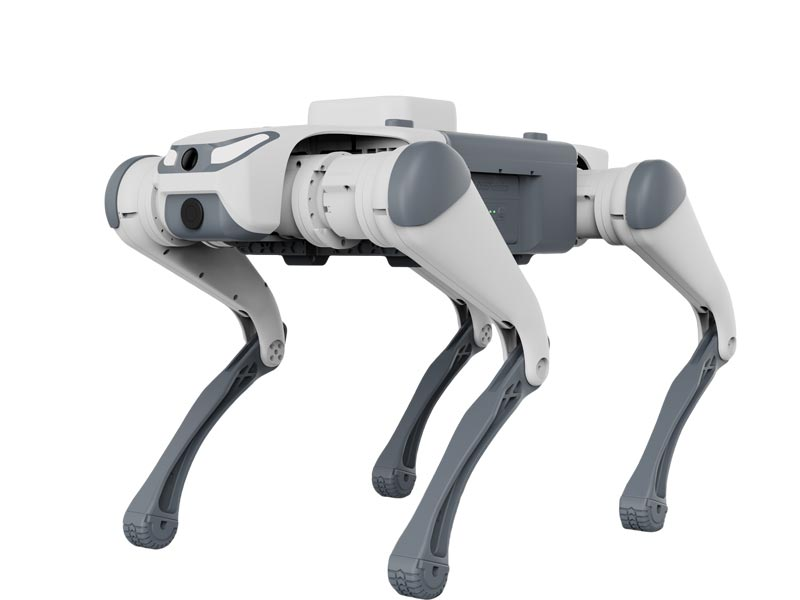
\includegraphics[scale=0.25]{gambar/quadruped_robot.jpg}
  \caption{DeepRobotics Lite3}
  \label{fig:quadruped_robot}
\end{figure}

Dalam hal desain dan kontrol, robot \emph{quadruped} mengadopsi prinsip-prinsip biomekanika
untuk meniru pola gerak alami hewan. Pola gerak ini, yang dikenal sebagai \emph{gait},
mencakup berbagai cara berjalan seperti \emph{trot}, \emph{pace}, dan \emph{gallop},
yang masing-masing digunakan tergantung pada kecepatan dan kondisi medan.
Implementasi gerakan ini membutuhkan sistem kendali yang kompleks,
termasuk algoritma keseimbangan dinamis dan kontrol koordinasi antar kaki.
Beberapa robot \emph{quadruped} menggunakan sensor inersia (IMU), kamera,
serta teknologi kecerdasan buatan (AI) untuk meningkatkan kesadaran situasional dan kemampuan navigasi secara otonom.

Robot \emph{quadruped} dapat dikategorikan berdasarkan sistem aktuasi yang digunakan,
yaitu robot dengan aktuasi elektrik, hidraulik, atau kombinasi keduanya.
Robot dengan aktuator elektrik cenderung lebih ringan dan lebih efisien dalam hal konsumsi daya,
sementara robot hidraulik lebih kuat dan mampu menangani beban yang lebih berat.
Beberapa robot \emph{quadruped} yang telah dikembangkan termasuk Spot dari Boston Dynamics,
ANYmal dari ANYbotics, dan Unitree Go1, yang digunakan dalam berbagai penelitian dan aplikasi industri.

Penggunaan robot \emph{quadruped} terus berkembang, terutama dalam bidang militer, eksplorasi luar angkasa,
pertanian, dan robotika layanan. Dengan kemampuannya untuk bergerak secara fleksibel di medan yang menantang
dan membawa beban tambahan, robot ini memiliki potensi besar untuk digunakan dalam
skenario di mana robot beroda atau berkaki dua mengalami kesulitan.
Tantangan utama dalam pengembangan robot \emph{quadruped} meliputi efisiensi energi, ketahanan perangkat keras,
dan peningkatan kecerdasan buatan agar mampu beradaptasi lebih baik dengan lingkungan yang tidak terstruktur.

\subsection{Robot Lengan}

\begin{figure} [H] \centering
  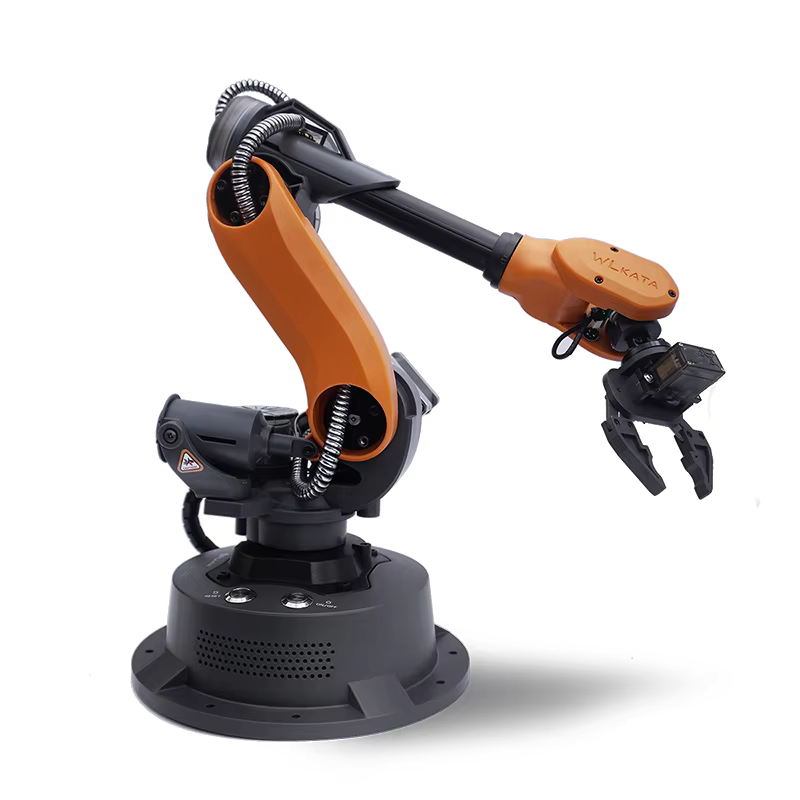
\includegraphics[scale=0.25]{gambar/arm_robot.png}
  \caption{Salah Satu Jenis Robot Lengan Dari Wlkata}
  \label{fig:arm_robot}
\end{figure}
Robot lengan, atau \emph{robotic arm}, adalah jenis robot yang dirancang untuk meniru fungsi lengan manusia
dalam melakukan berbagai tugas manipulasi objek. Robot ini umumnya terdiri dari serangkaian sambungan (\emph{joints})
dan batang (\emph{links}) yang memungkinkan pergerakan fleksibel dalam berbagai arah. Dengan kombinasi aktuator,
sensor, dan sistem kendali yang kompleks, robot lengan mampu melakukan tugas-tugas seperti \emph{pick-and-place},
perakitan, pengelasan, pengecatan, serta tugas presisi lainnya dalam industri manufaktur, medis, dan penelitian.

Robot lengan dapat dikategorikan berdasarkan konfigurasi kinematiknya, seperti robot kartesian,
robot SCARA (\emph{Selective Compliance Articulated Robot Arm}), robot artikulasi, dan robot delta.
Robot kartesian memiliki tiga derajat kebebasan dalam sumbu X, Y, dan Z, serta sering digunakan
dalam aplikasi yang membutuhkan pergerakan linier, seperti mesin CNC. Robot SCARA memiliki fleksibilitas
lebih dalam bidang horizontal dan umumnya digunakan dalam proses perakitan cepat. Robot artikulasi,
yang memiliki sambungan berputar serupa dengan lengan manusia, digunakan dalam berbagai aplikasi industri
dan medis karena kemampuannya untuk mencapai berbagai sudut dan melakukan gerakan yang kompleks.
Sementara itu, robot delta, yang memiliki struktur paralel, biasanya diterapkan dalam industri makanan
dan farmasi untuk tugas-tugas kecepatan tinggi dengan presisi tinggi.

Dalam implementasi teknologinya, robot lengan menggunakan berbagai sensor dan aktuator untuk
meningkatkan akurasi dan efisiensi operasional\parencite{ZhenXie_lbrgar}. Sensor posisi dan kecepatan digunakan untuk
mengontrol gerakan sendi, sementara sensor gaya dan torsi memungkinkan robot berinteraksi
dengan lingkungan secara lebih presisi, misalnya dalam tugas perakitan yang membutuhkan kepekaan
terhadap perubahan gaya. Kamera dan sistem visi komputer juga sering digunakan untuk mendeteksi
dan mengenali objek, memungkinkan robot melakukan tugas-tugas berbasis kecerdasan buatan
seperti penyortiran otomatis dan inspeksi kualitas produk.

Sistem kendali robot lengan dapat dibagi menjadi kontrol terbuka (\emph{open-loop control}) dan
kontrol tertutup (\emph{closed-loop control}). Dalam sistem kontrol terbuka, perintah gerakan diberikan
tanpa umpan balik dari sensor, sementara dalam kontrol tertutup, sistem terus memantau dan
menyesuaikan gerakan berdasarkan informasi dari sensor, sehingga menghasilkan pergerakan
yang lebih akurat dan adaptif. Algoritma kendali seperti \emph{PID control}, \emph{inverse kinematics},
dan \emph{reinforcement learning} sering digunakan untuk meningkatkan performa robot dalam
menyesuaikan gerakan terhadap tugas tertentu.

Robot lengan telah menjadi bagian penting dalam revolusi industri dan otomatisasi modern.
Dalam industri manufaktur, robot ini digunakan untuk meningkatkan produktivitas dan
mengurangi risiko cedera pada pekerja manusia. Di bidang medis, robot bedah seperti
da Vinci Surgical System memungkinkan prosedur bedah yang lebih presisi dan minim invasif.
Selain itu, dalam dunia penelitian dan eksplorasi luar angkasa, robot lengan digunakan
dalam eksperimen ilmiah dan misi eksplorasi, seperti lengan robotik yang dipasang pada \emph{rover} penjelajah Mars.

\subsection{Human-Robot Interaction}

Interaksi manusia-robot (\emph{Human-Robot Interaction}) adalah bidang multidisiplin yang berfokus
pada cara manusia dan robot berkomunikasi, bekerja sama, serta berbagi lingkungan dalam berbagai konteks aplikasi.
Dengan semakin berkembangnya teknologi robotika, interaksi antara manusia dan robot tidak lagi
terbatas pada pengoperasian manual di lingkungan industri, tetapi juga meluas ke bidang kesehatan, layanan pelanggan,
edukasi, hingga penggunaan dalam kehidupan sehari-hari. Oleh karena itu, desain dan pengembangan sistem interaksi yang intuitif,
aman, serta efisien menjadi aspek yang sangat penting dalam penelitian dan implementasi robotika modern.

HRI dapat dikategorikan berdasarkan tingkat keterlibatan manusia dalam pengendalian robot, yaitu \emph{remote interaction},
\emph{supervisory control}, \emph{collaborative interaction}, dan \emph{fully autonomous interaction}. Dalam \emph{remote interaction}, manusia
mengendalikan robot dari jarak jauh, misalnya dalam operasi militer atau eksplorasi luar angkasa. Pada \emph{supervisory control},
manusia memberikan instruksi tingkat tinggi sementara robot mengeksekusi tugasnya secara semi-otomatis, seperti dalam sistem
robot bedah atau kendaraan otonom. Dalam \emph{collaborative interaction}, manusia dan robot bekerja berdampingan, seperti di pabrik
manufaktur yang menerapkan cobots (\emph{collaborative robots}). Sementara itu, dalam \emph{fully autonomous interaction}, robot dapat
beroperasi secara mandiri dengan pemahaman penuh terhadap lingkungan dan kebutuhan manusia, seperti asisten rumah tangga
berbasis kecerdasan buatan.

\begin{figure} [H] \centering
    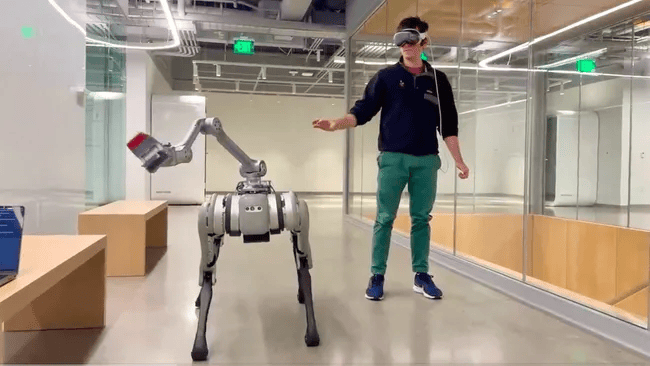
\includegraphics[scale=0.4]{gambar/HRI daster.png}
    \caption{Salah Satu Bentuk Interaksi Supervisory Control\parencite{img_HRI}}
    \label{fig:HRI_daster}
\end{figure}

Salah satu tantangan utama dalam HRI adalah pengembangan sistem komunikasi yang efektif antara manusia dan robot\parencite{QifanZhang_tlihrifamoagdwqr}.
Metode komunikasi ini bisa berupa antarmuka fisik seperti tombol dan \emph{joystick}, antarmuka berbasis suara (\emph{speech recognition}),
bahasa tubuh, serta ekspresi wajah yang dapat dikenali oleh robot menggunakan sistem visi komputer. Dalam beberapa sistem,
robot dapat memahami emosi manusia dengan mendeteksi ekspresi wajah dan intonasi suara, memungkinkan interaksi yang lebih alami dan
intuitif. Sebagai contoh, robot sosial seperti Pepper dan NAO dirancang untuk memahami dan merespons interaksi manusia dengan cara
yang lebih mirip interaksi antarmanusia. Keamanan dan kepercayaan juga menjadi faktor krusial dalam interaksi manusia-robot,
terutama dalam lingkungan di mana robot bekerja berdampingan dengan manusia. Penggunaan sensor dan algoritma kecerdasan buatan
memungkinkan robot untuk mengenali dan merespons keberadaan manusia di sekitarnya secara aman. Misalnya, robot kolaboratif yang
digunakan dalam industri manufaktur sering kali dilengkapi dengan sensor gaya dan torsi untuk mendeteksi adanya hambatan fisik,
sehingga dapat memperlambat atau menghentikan gerakan ketika mendekati manusia. Selain itu, desain robot yang lebih ramah secara
visual dan ergonomis dapat meningkatkan kepercayaan pengguna terhadap teknologi ini.  

\begin{figure} [H] \centering
    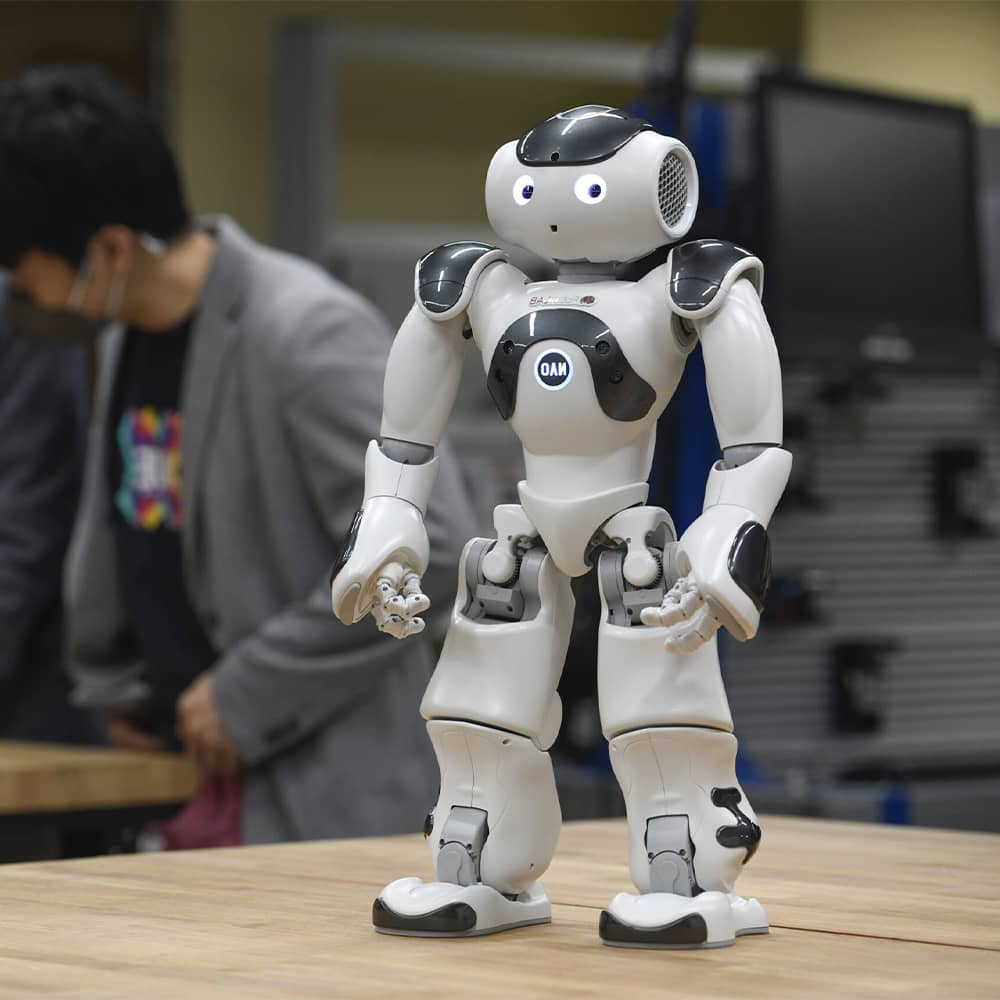
\includegraphics[scale=0.2]{gambar/NAO_robot.jpg}
    \caption{Salah Satu Contoh Robot Sosial NAO}
    \label{fig:HRI_NAO_daster}
\end{figure}

Dalam bidang kesehatan, HRI memainkan peran penting dalam pengembangan robot pendamping bagi lansia atau pasien dengan kebutuhan khusus.
Robot semacam ini dapat membantu dalam aktivitas sehari-hari, memberikan pengingat untuk minum obat, atau bahkan menyediakan interaksi
sosial bagi pengguna yang mengalami kesepian. Selain itu, dalam terapi anak-anak dengan autisme, robot telah digunakan untuk membantu
meningkatkan keterampilan sosial mereka dengan interaksi yang lebih konsisten dan dapat diprediksi dibandingkan dengan manusia.  
Seiring dengan meningkatnya penggunaan robot dalam berbagai aspek kehidupan, tantangan etika dalam HRI juga menjadi perhatian utama.
Isu-isu seperti privasi data pengguna, pengaruh robot terhadap tenaga kerja manusia, serta batasan dalam interaksi emosional antara
manusia dan robot menjadi bahan diskusi yang terus berkembang.

\subsection{Grasping Pose Detection}

\emph{Grasping pose detection} adalah bidang yang berfokus pada pengenalan dan
penentuan posisi optimal bagi robot untuk mengambil, memegang, dan memanipulasi objek dengan tangannya atau
\emph{end-effector}. \emph{Grasping pose detection} merupakan aspek krusial dalam sistem robotik, terutama
pada aplikasi seperti otomatisasi industri, layanan rumah tangga, logistik, serta bidang kesehatan. Kemampuan
robot untuk secara akurat menentukan bagaimana cara menggenggam suatu objek sangat bergantung pada berbagai
faktor seperti bentuk, ukuran, tekstur, dan material dari objek tersebut, serta kondisi lingkungan sekitarnya\parencite{ZhenXie_lbrgar}.

\emph{Grasping pose detection} sering kali mengandalkan kombinasi antara teknologi sensor, algoritma, serta kecerdasan buatan.
Sensor yang umum digunakan meliputi kamera RGB, kamera \emph{depth}, sensor LiDAR, dan sensor sentuh (\emph{tactile sensor}).
Kamera RGB-D, seperti Intel RealSense atau Microsoft Kinect, memungkinkan robot untuk menangkap informasi visual serta kedalaman objek,
sehingga dapat memahami bentuk tiga dimensi dari objek yang akan digenggam. Sementara itu, sensor sentuh memberikan umpan balik langsung
tentang tekanan dan gesekan yang diterapkan oleh gripper robot terhadap objek yang dipegang, memungkinkan penyesuaian genggaman secara
\emph{real-time} untuk menghindari tergelincir atau merusak objek.
Algoritma yang digunakan dalam \emph{Grasping Pose Detection} umumnya memanfaatkan teknik pengolahan citra dan pembelajaran mesin.
Pendekatan berbasis visi komputer sering kali menggunakan teknik seperti \emph{edge detection}, \emph{feature extraction}, dan segmentasi objek
untuk mengidentifikasi kontur serta titik-titik kritis pada objek. Dengan kemajuan kecerdasan buatan, terutama \emph{deep learning}, banyak
penelitian telah mengembangkan model berbasis jaringan saraf konvolusional (\emph{Convolutional Neural Networks} atau CNN) serta model
berbasis \emph{Reinforcement Learning} untuk mempelajari strategi genggaman yang lebih fleksibel dan adaptif.
Selanjutnya, metode berbasis \emph{motion planning} digunakan untuk membantu robot lengan dalam
merancang lintasan yang optimal sehingga robot dapat mencapai posisi genggaman tanpa menabrak rintangan di sekitarnya.
Metode ini sering dikombinasikan dengan pendekatan berbasis \emph{inverse kinematics} untuk menghitung konfigurasi sendi yang
memungkinkan robot mencapai target genggaman dengan sudut dan orientasi yang sesuai.

\begin{figure} [H] \centering
    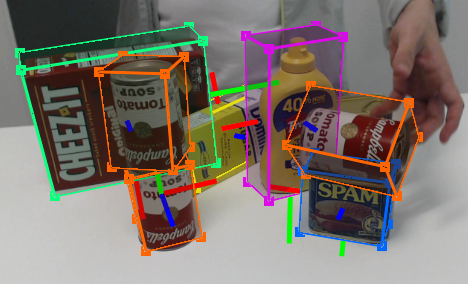
\includegraphics[scale=0.95]{gambar/grasping_pose_detection.png}
    \caption{Hasil Riset NVIDIA dalam pemanfaatan deep learning untuk grasping robot\parencite{img_grasping_daster}}
    \label{fig:grasping_daster}
\end{figure}

Salah satu tantangan utama dalam \emph{Grasping Pose Detection} adalah menghadapi objek dengan bentuk yang kompleks,
permukaan yang reflektif, atau kondisi pencahayaan yang berubah-ubah. Selain itu, keberadaan lingkungan yang dinamis,
seperti objek yang bergerak atau berubah posisinya, juga menambah kompleksitas dalam menentukan strategi genggaman
yang optimal.
Dalam aplikasi nyata, \emph{Grasping Pose Detection} telah digunakan dalam berbagai bidang,
seperti robot pemindah barang di gudang \emph{e-commerce}, sistem asisten robotik di rumah tangga,
hingga robot medis yang dapat memegang dan memanipulasi peralatan bedah dengan presisi tinggi.

\subsection{Pengolahan Citra}
Dalam suatu sistem komputasi, citra yang ditemui pada dunia nyata tidak dapat secara
langsung direpresentasikan oleh komputer. Dalam merubah bentuk citra di dunia nyata atau
yang sering disebut citra analog perlu dilakukan perubahan dengan menggunakan sistem \emph{sampling}.
Sistem \emph{sampling} ini berguna untuk mengubah citra analog menjadi M baris N kolom dan
hasil ini dapat didefinisikan sebagai citra diskrit. Pertemuan titik antara M baris dan N kolom
ini dinamakan dengan Piksel atau titik terkecil dari sebuah citra digital. Selain sistem \emph{sampling},
di dalam citra digital juga terdapat kuantisasi. Kuantitasi adalah sebuah pemberian nilai-nilai
tertentu pada sebuah piksel di dalam citra digital. Nilai kuantisasi ini dapat merepresentasikan
warna maupun kecerahan dari piksel di dalam sebuah citra digital.

Dengan adanya piksel dan hasil nilai kuantisasi maka dapat dilakukan pengoperasian matematika pada nilai kuantisasi
di seluruh piksel yang dimiliki sebuah citra digital. Salah satu cara pengolahan yang paling mudah adalah dengan
menggunakan \emph{library} yang bernama OpenCV\parencite{RDKusumanto_pcdumompwmnr}. OpenCV mampu membantu dalam pemrosesan
data nilai suatu gambar yang dimana di dalam komputer hasil dari \emph{sampling} dan kuantisasi ini direpresentasikan
sebagai sebuah \emph{array}. Pengolahan citra sering digunakan untuk mempersiapakan gambar sebelum diolah oleh program
\emph{machine learning} sehingga menghasilkan hasil keputusan yang jauh lebih baik dibandingkan langsung memberikan gambar.

Pengolahan citra memainkan peran penting dalam operasi robot lengan, terutama dalam meningkatkan akurasi
dan efisiensi manipulasi objek dalam berbagai lingkungan. Dengan menggunakan kamera sebagai sensor visual, robot lengan
dapat memperoleh informasi mengenai posisi, orientasi, serta karakteristik objek yang akan dipegang atau dipindahkan.
Teknologi pengolahan citra memungkinkan robot untuk mendeteksi dan mengenali objek, mengklasifikasikan bentuk dan warna,
serta menyesuaikan gerakan lengan agar sesuai dengan kondisi lingkungan.

\subsection{ROS}
\emph{Robot Operating System} (ROS) adalah sebuah \emph{framework open-source} yang dirancang untuk mendukung pengembangan
perangkat lunak robotika yang kompleks dan modular. Meskipun namanya mengandung kata "\emph{Operating System}," ROS
sebenarnya bukanlah sistem operasi yang independen, melainkan sebuah \emph{middleware} yang berjalan di atas sistem operasi
seperti Ubuntu (Linux) dan menyediakan berbagai \emph{tools} serta \emph{library} untuk membantu \emph{developer} dalam membangun
aplikasi robotika. ROS dikembangkan oleh Willow Garage dan sejak itu telah berkembang menjadi standar industri
dalam komunitas robotika, baik dalam lingkungan akademik maupun industri.

\begin{figure} [H] \centering
    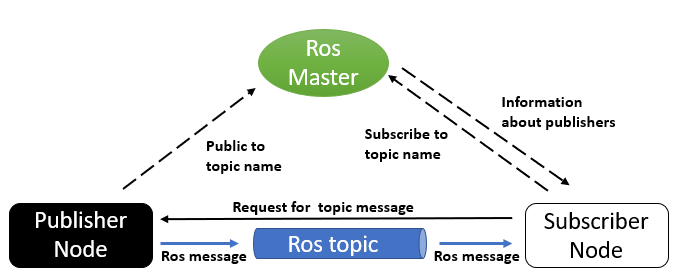
\includegraphics[scale=0.65]{gambar/ros_system.png}
    \caption{Sistem Kerja ROS\parencite{img_ros_system}}
    \label{fig:ros_system}
\end{figure}

Salah satu keunggulan utama ROS adalah arsitektur berbasis \emph{node} dan komunikasi antarproses\parencite{ros_website}. Dalam ROS,
sebuah sistem robot dapat dibagi menjadi beberapa \emph{node}, di mana setiap \emph{node} bertanggung jawab untuk menjalankan tugas
tertentu, seperti pemrosesan sensor, kendali aktuator, atau perencanaan gerak. tiap-tiap \emph{node} ini dapat berkomunikasi
satu sama lain menggunakan ROS \emph{topics}, \emph{services}, dan \emph{actions}, yang memungkinkan sistem menjadi lebih modular dan
fleksibel. Misalnya, sebuah \emph{mobile robot} yang menggunakan kamera dan LIDAR untuk navigasi dapat memiliki satu \emph{node}
untuk pemrosesan citra, satu \emph{node} untuk pemetaan lingkungan, dan satu \emph{node} untuk pengendalian gerak, yang semuanya
bekerja secara terpisah tetapi tetap dapat saling bertukar informasi.
Salah satu fitur penting lain dalam ROS adalah dukungan terhadap sistem terdistribusi, yang memungkinkan
beberapa komputer untuk bekerja secara bersama-sama dalam satu jaringan ROS. Hal ini sangat berguna dalam
sistem robotik yang kompleks, misalnya pada robot otonom yang terdiri dari beberapa subsistem terpisah
seperti robot lengan yang bekerja bersama dengan \emph{mobile robot}.

Selain itu, ROS menyediakan berbagai \emph{library} yang telah dioptimalkan untuk pemrosesan sensor,
SLAM (\emph{Simultaneous Localization and Mapping}), perencanaan gerak, kontrol robotik, dan visi komputer.
Salah satu \emph{library} yang sering digunakan dalam ROS adalah MoveIt!, yang mendukung perencanaan gerak
pada robot manipulator seperti lengan robot. Selain itu, ada juga \emph{library} seperti OpenCV untuk
pemrosesan citra, PCL untuk pemrosesan data 3D dari LIDAR, serta integrasi dengan
berbagai jenis sensor dan aktuator melalui \emph{driver} yang telah dikembangkan dalam komunitas ROS.
ROS juga mendukung simulasi robot melalui integrasi dengan Gazebo, RViz, dan simulasi berbasis \emph{physics engine} lainnya.
Gazebo memungkinkan \emph{developer} untuk menguji algoritma kontrol robot dalam lingkungan simulasi sebelum diterapkan pada
perangkat keras nyata, yang sangat berguna untuk menghindari kerusakan pada robot akibat kesalahan pemrograman. RViz,
di sisi lain, adalah alat visualisasi yang digunakan untuk menampilkan data sensor, trajektori robot, serta hasil dari
berbagai algoritma pemrosesan yang berjalan di dalam sistem ROS.

\subsection{GraspNet}

\subsection{QT}